\chapter{Fitting experimental data}
Related YouTube videos:
\begin{figure}[H]

\begin{tabular}{ c l }


\includegraphics[width=0.05\textwidth]{./images/youtube.png}

&
\href{https://www.youtube.com/watch?v=uEj0dB-mPTQ}{Advanced topics in fitting of JV curves to experimental data using \simname.}\
\\

\includegraphics[width=0.05\textwidth]{./images/youtube.png}

&
\href{https://www.youtube.com/watch?v=WY_grICDP4Y}{Fitting transient photocurrent (TPC) and light JV curves using \simname}
\\

\includegraphics[width=0.05\textwidth]{./images/youtube.png}

&
\href{https://www.youtube.com/watch?v=61umU4hrsqk&t=58s}{Fitting the light JV curve of an ultra large area (2.5meter x 1cm) OPV device using \simname}

\end{tabular}
\end{figure}

\label{sec:fitting}
In the same way you can fit the diode equation to a dark curve of a solar cell to extract the ideality factor, OghmaNano can be fit to experimental data using the fitting function. Fitting is a good way to extract physical parameters from a device such as mobility, destiny of trap states etc. The advantage of fitting a complex model such as OghmaNano to data rather than simplistic analytical equations is that far more detailed information can be extracted and a better physical picture of the underlying physics obtained. This section gives an overview of the fitting tools in OghamNano.

\section{Key tips and tricks}
\label{sec:key_tips_and_tricks}

\begin{itemize}
  \item Generally speaking fitting is tricky process requiring a lot of patience and manual fine tuning to get it to work. Don't expect to click a button and for it to just work. You will have to work to get nice fits.

  \item If the fit is not working something may be wrong with the physical assumptions you have made with your device. The model will only fit physically reasonable data so if something is off by and order of magnitude go back and think again about what you are asking the model to do. For example if you just can't get $J_{sc}$ to match on a solar cell, could it be that your material just just not absorbing enough photons to get your desired $J_{sc}$ value?

  \item Different data sets provide different types of information. For example the dark JV curve of a solar cell provides information about the shunt resistance, the series resistance, and some information about mobility and recombination/tale states. However, the light JV curve provides almost no information about the shunt resistance so don't expect a fit to the light JV curve to provide accurate estimates of $R_{shunt}$. Alway think about what information is contained within your data before interpreting the numbers extracted from a fit.

  \item The fitting works process by: 1) Running a simulation; 2) Calculating the difference between the numerical and experimental results; 3) tweaking the simulation parameters ; 4) rerunning the simulation and seeing if the difference between the experiment and simulation has reduced; 5) If the error has reduced the change of parameter is accepted and the process repeated with a different parameter.  This process continues hundreds or thousands of times until an acceptable fit has been achieved. Therefore, to do a fit the model must be run thousands of times, this means that for a fit to arrive at an answer quickly, the individual simulation when run alone must be fast. So for example if your simulation has 1000 mesh points, when fitting try reducing this to 10. Or if you have 1000 time steps try reducing this to 100. Every speed up in the base simulation will result in a speed up in the fitting process.

  \item Writing files to disk is the slowest part of any computational process. Even modern SSDs are about 30 times slower than main memory for example the maximum write speed to an SSD is 456 MB/s where as the bandwidth of a PC3-12800 memory module is  12,800 MB/s. When you save your files on USB drives, network storage drives, or even worse the internet aka OneDrive or Dropbox, read write speeds again drop massively. Therefore if you want your simulation to run fast save it on a local hard disk which is ideally and SSD and not a mechanical drive and not being mirrored over the network.

  \item As stated above writing files to disk is slow, therefore try to minimize the number of files your simulation kicks out. Turn off things such as snapshots, optical output and the dynamic folder.  You can check if your simulation is dumping a lot of files by opening your simulation directory in windows explorer and counting the files.  A simulation set to write very little to disk should have about 50 files in it. If your simulation directory has hundreds of files in it then you need to find out why.

 \item Although you can fit with the GUI, it can be slow. I personally tend to set up fits in the GUI but run them from the command line. There is a section on how to do this below.

 \item Fitting writes quite a lot of files to disk. Virus killers can slow down the fitting significantly as they scan all the data files before they are written to disk.   
\end{itemize}

\section{The main fitting window}

An example of how to fit the model to experimental data is included in the demo simulations provided with OghmaNano. In this example a simple drift diffusion model is fit to some experimental data. If you click on the \emph{New simulation} icon in the File ribbon, this will bring the new simulation window as seen in Figure \ref{fig:fit_new_sim}a. Double click on the \emph{Scripting and fitting} icon, this will display the menu that can be seen in Figure \ref{fig:fit_new_sim}b. From this menu double click on the  \emph{Fitting and parameter extraction} example.(see \ref{fig:fit_new_sim}a). If you open this simulation you will be presented with the window shown in Figure (see \ref{fig:fit_main_window}), this is a simple solar cell simulation. It should be noted that the fitting engine can be used to fit any simulation to any data set.


\begin{figure}[H]
\centering
\begin{tabular}{ c c }

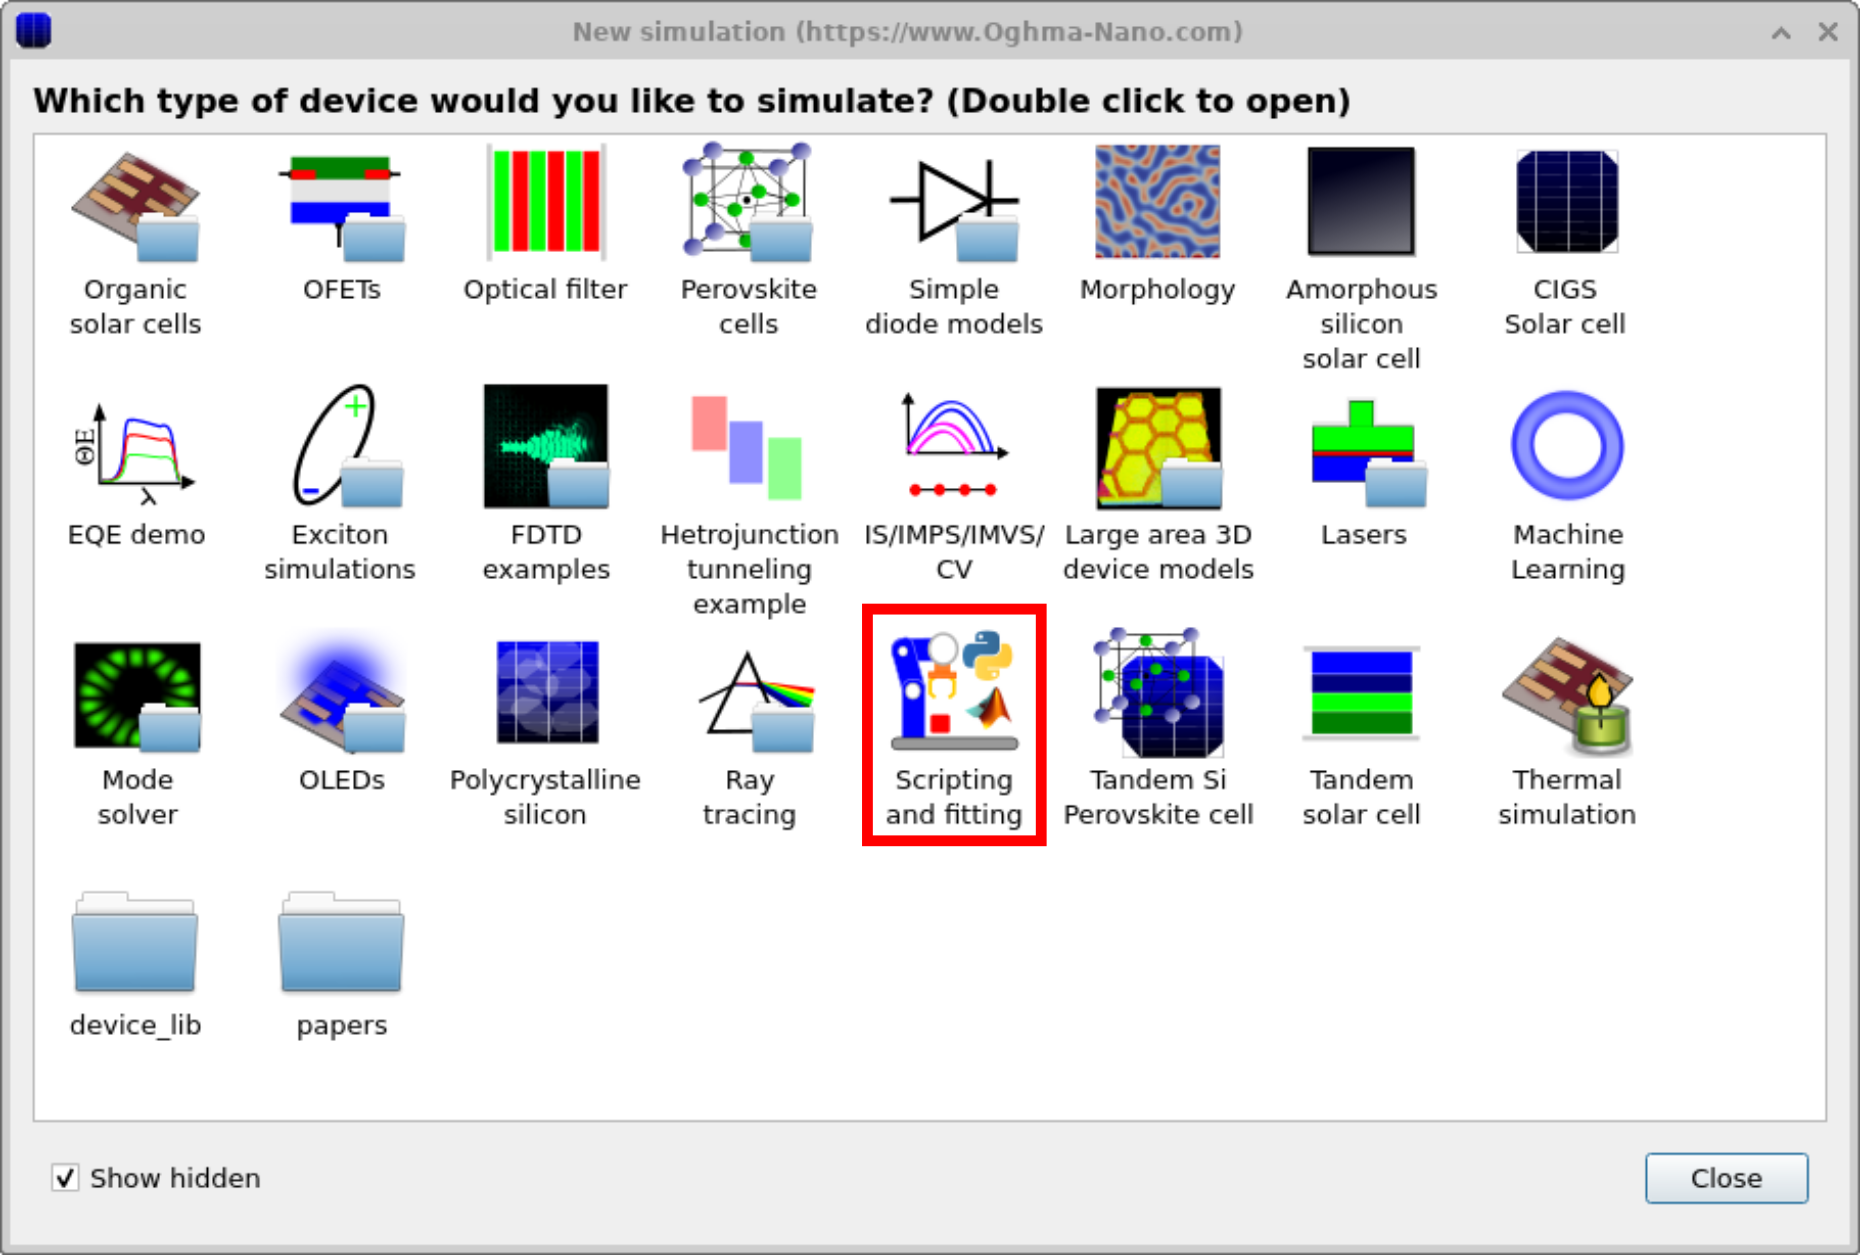
\includegraphics[width=0.45\textwidth]{./images/fit/example.png}
&
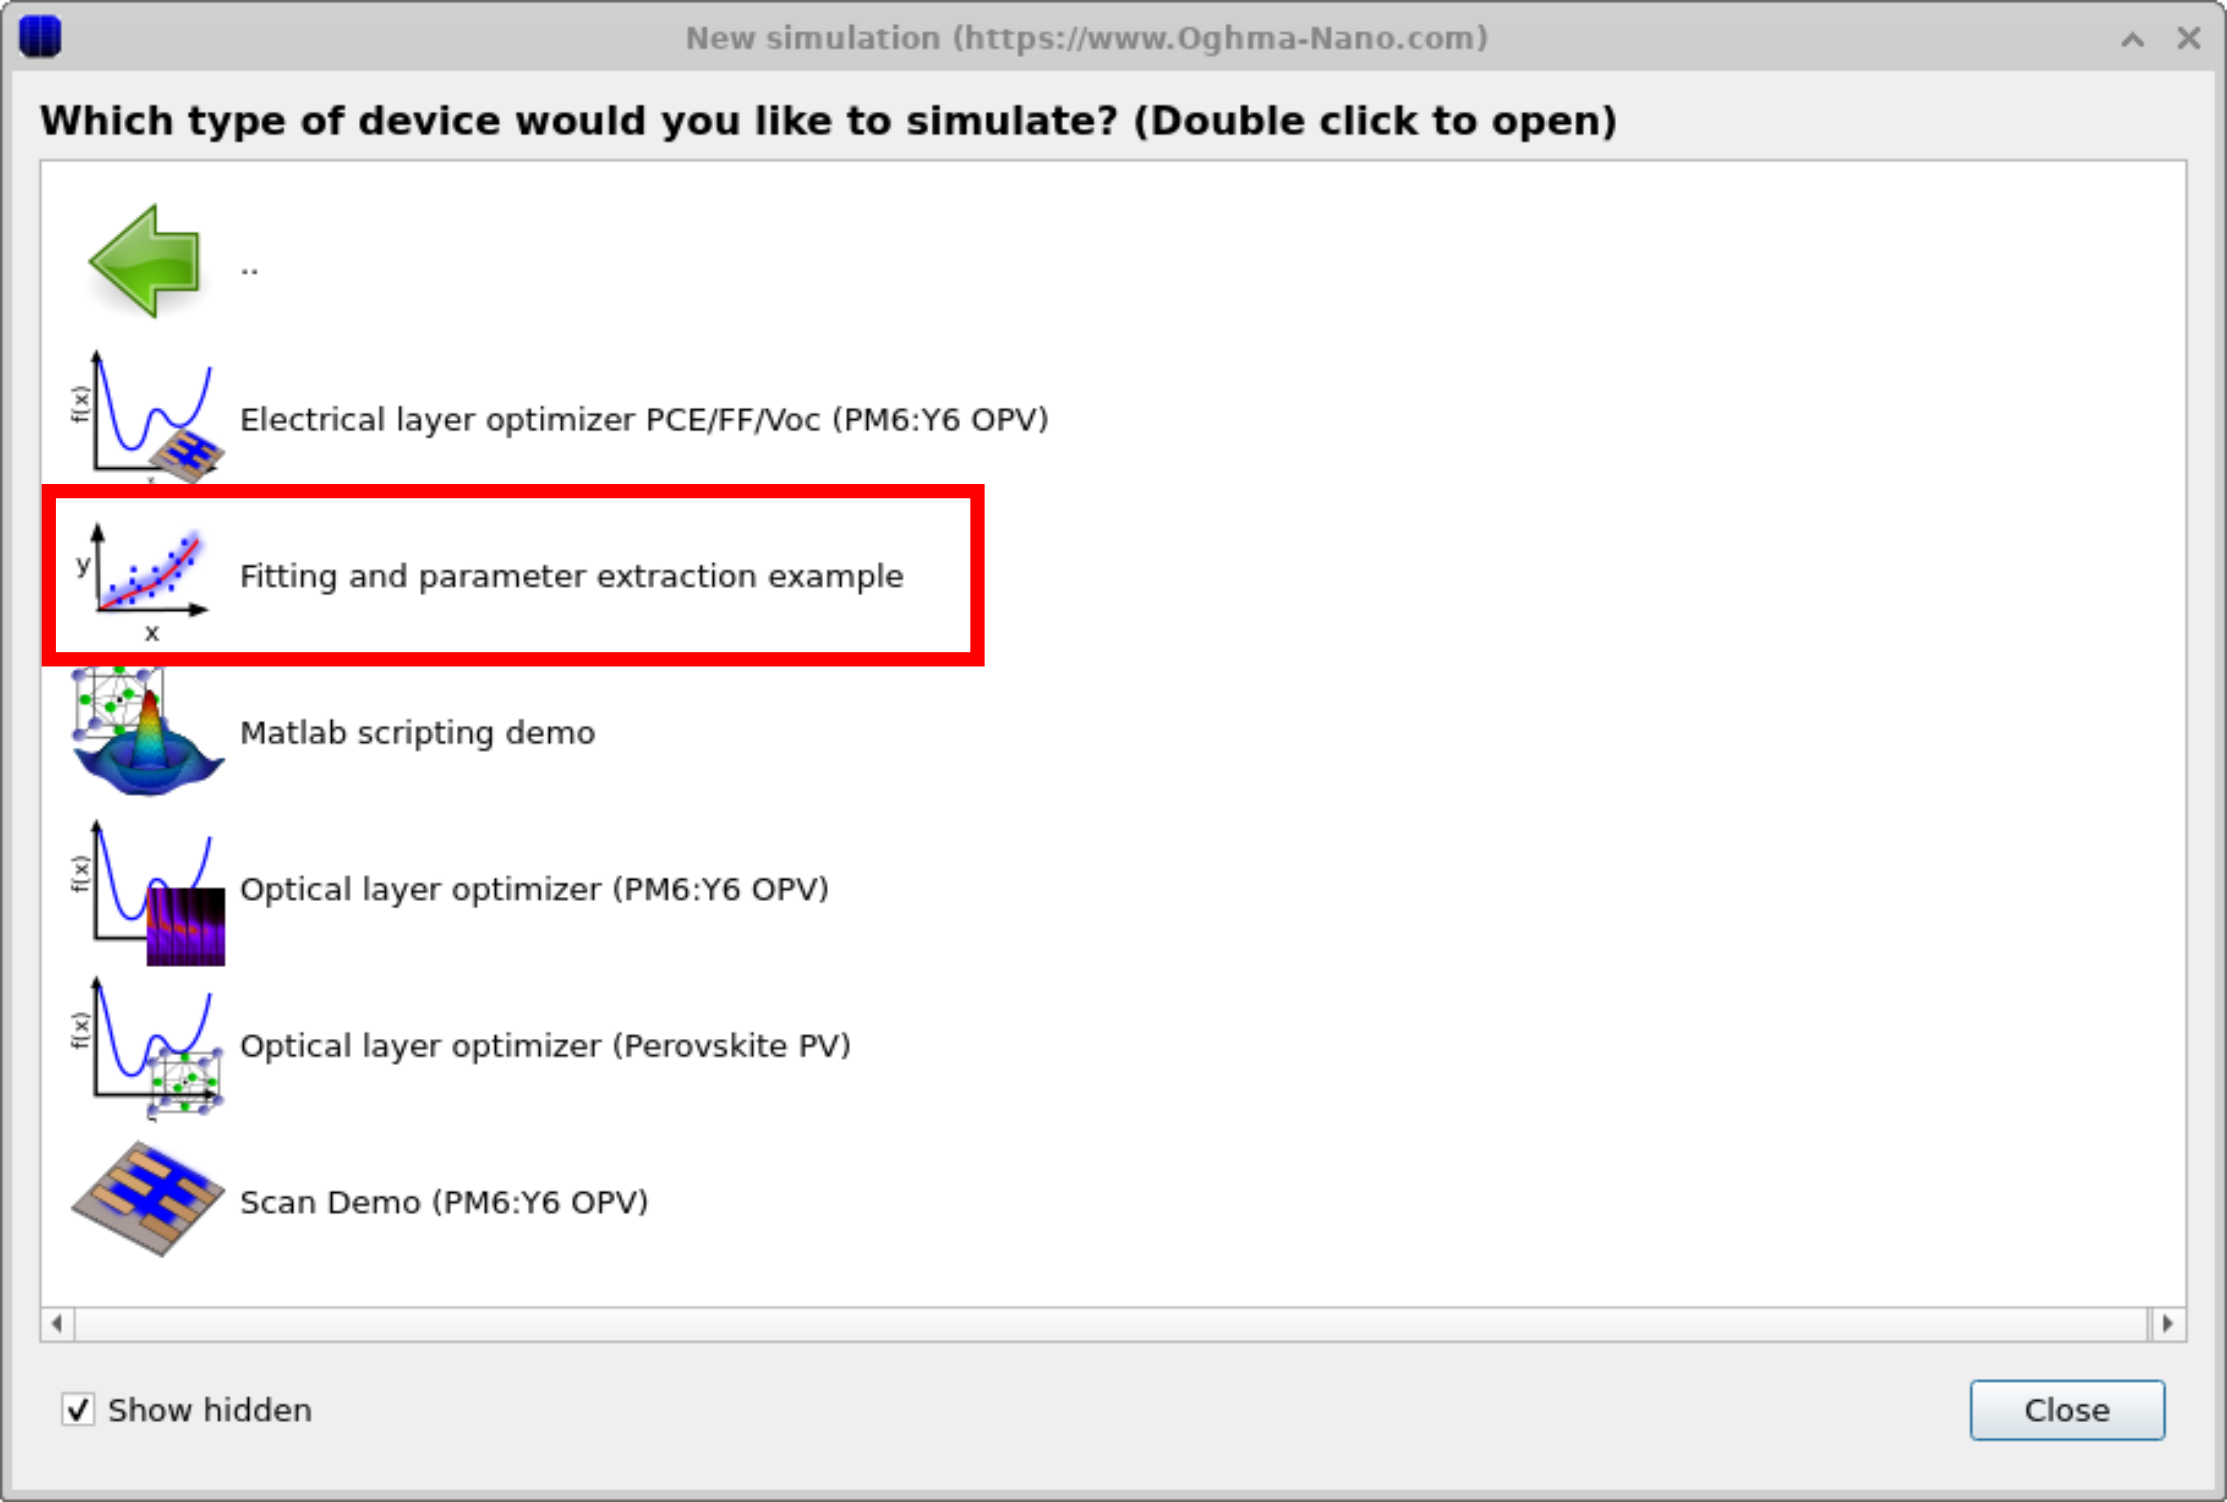
\includegraphics[width=0.45\textwidth]{./images/fit/example1.png}
\\
\end{tabular}
\caption{a) The example fitting simulation can be found in the \emph{Scripting and fitting} folder b) The fitting example is called \emph{Fitting and parameter extraction example}.}
\label{fig:fit_new_sim}
\end{figure}

\begin{figure}[H]
\centering
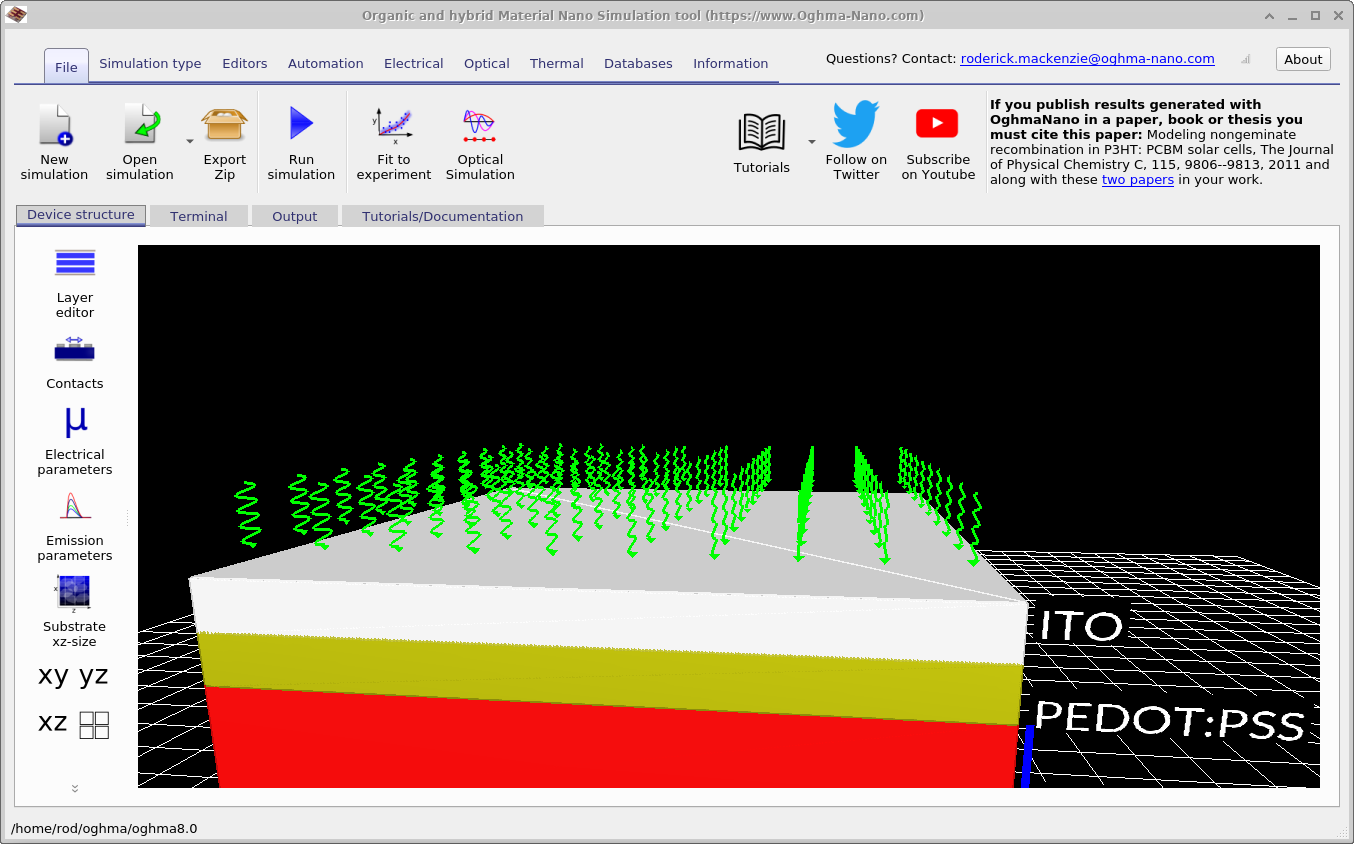
\includegraphics[width=0.7\textwidth]{./images/fit/main_window.png}
\caption{The main fitting window.}
\label{fig:fit_main_window}
\end{figure}

\begin{figure}[H]
\centering
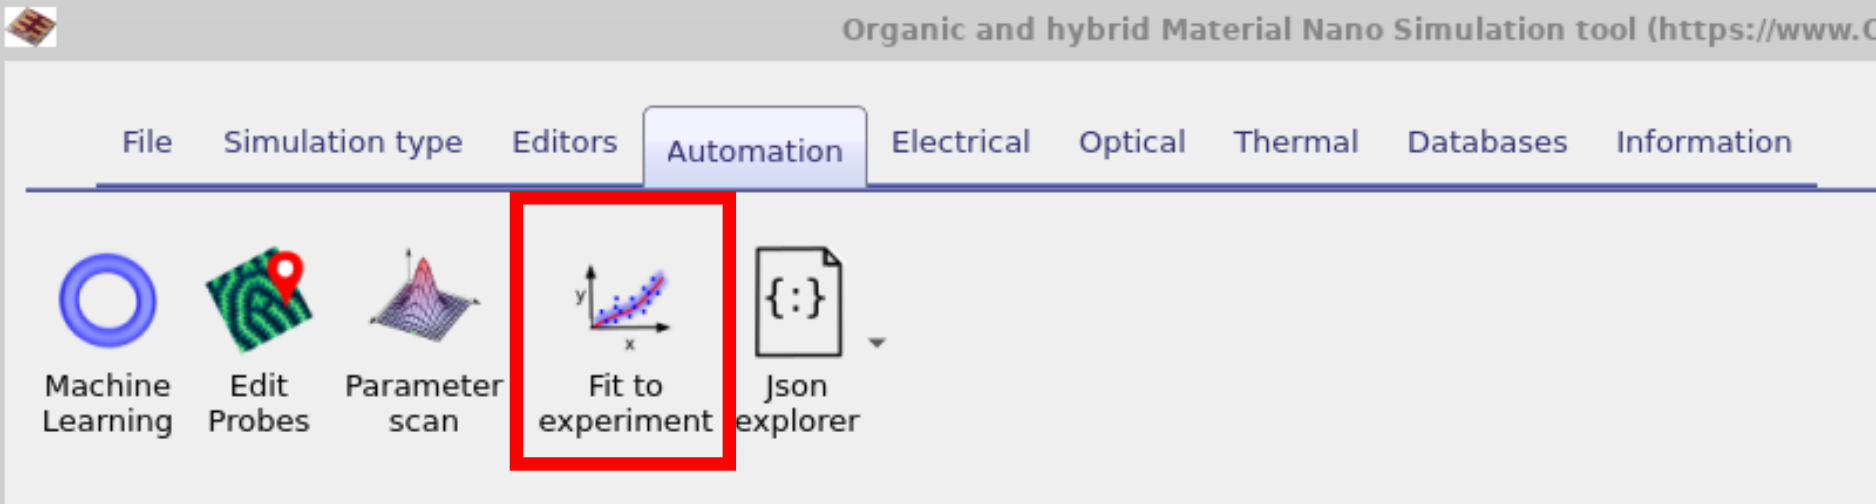
\includegraphics[width=0.7\textwidth]{./images/fit/main_fit_ribbon.png}
\caption{The fitting window can be accessed through the \emph{Automation} ribbon, using the \emph{Fit to experiment} icon.}
\label{fig:fit_main_ribbon}
\end{figure}

From the \emph{Automation} ribbon in the simulation (Figure \ref{fig:fit_main_ribbon}), click on the \emph{Fit to experiment} icon. This will bring up the fitting window (see figure \ref{fig:fit_window_first_open}).  The icons in the ribbon of the fitting window perform the following tasks:

\begin{itemize}
  \item New experiment: Currently the window is only displaying one set of experimental data in this case a light JV curve. Using the New experiment button one can add other data sets such as a dark JV curve to the fit. The more sets of data you fit against the more accurate your extracted parameters will be but the harder the fit will be to perform and the slower it will run.
  \item Delete experiment: This will remove a data set from the fit.
  \item Clone experiment: This will clone the current data set to a new data set.
  \item Rename experiment: This will rename the data set.
  \item Export data: This will export the fit to a zip file.
  \item Import data: This will import experimental data. The import wizard is explained elsewhere.
  \item Configure: This is used to configure the fitting variables, this is explained in detail below.
  \item One iteration data: This will run the fit just once to see how close to the experimental data it is. It is highly recommended to use this function and change the parameters by hand to get a closish fit before running the automated fit.
  \item Run fit: This will run the automated fitting algorithm. It will run forever, you have to press the button again to stop it.
  \item Fit this data set: This enables or disables the fitting of the data set currently being viewed.
\end{itemize}


\begin{figure}[H]
\centering
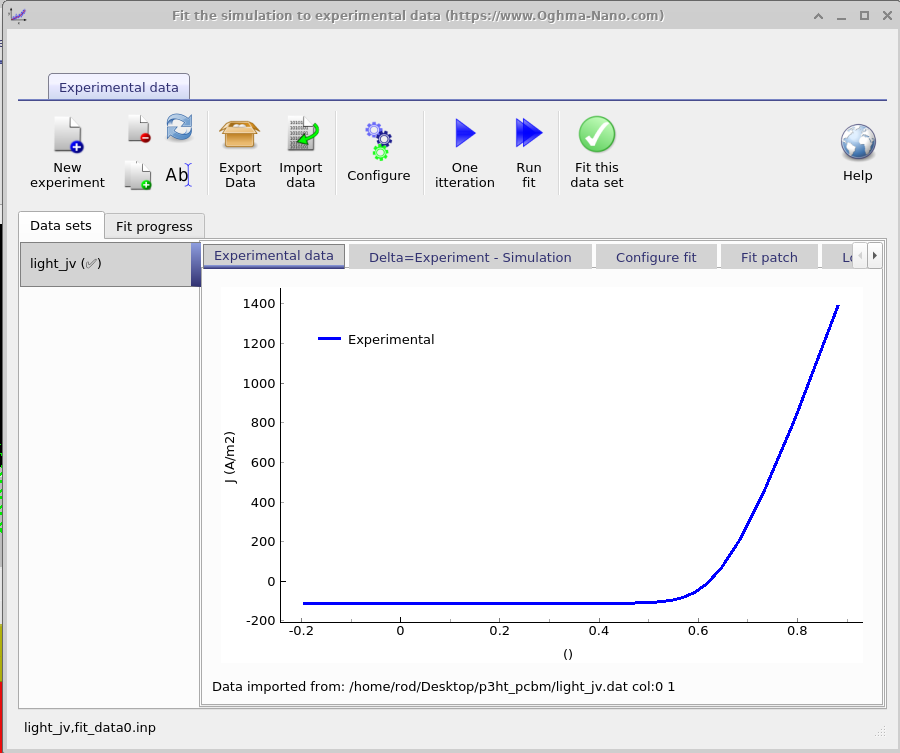
\includegraphics[width=0.7\textwidth]{./images/fit/fit_window_first_open.png}
\caption{The main fitting window.}
\label{fig:fit_window_first_open}
\end{figure}

If you click the one fit button, the fit window will update and will look like \ref{fig:fit_one_fit}a. You can now see the difference between the experimental and simulated curves.  The green line represents the difference between the two curves, it is called the error function. It represents the mathematical difference between the simulated and experimental data.  If you now click \emph{Run fit} to start the fitting process, you should see the curves gradually start to get closer and the error function decrease in value. Now click on the \emph{Fit progress} tab, this plots the error function as a function of fit iterations.  Watch as the error drops off. It should start looking like figure \ref{fig:fit_one_fit}b.  This process should take about 30 seconds, if it takes longer read section \ref{sec:key_tips_and_tricks} above.

\begin{figure}[H]
\centering
\begin{tabular}{ c c }

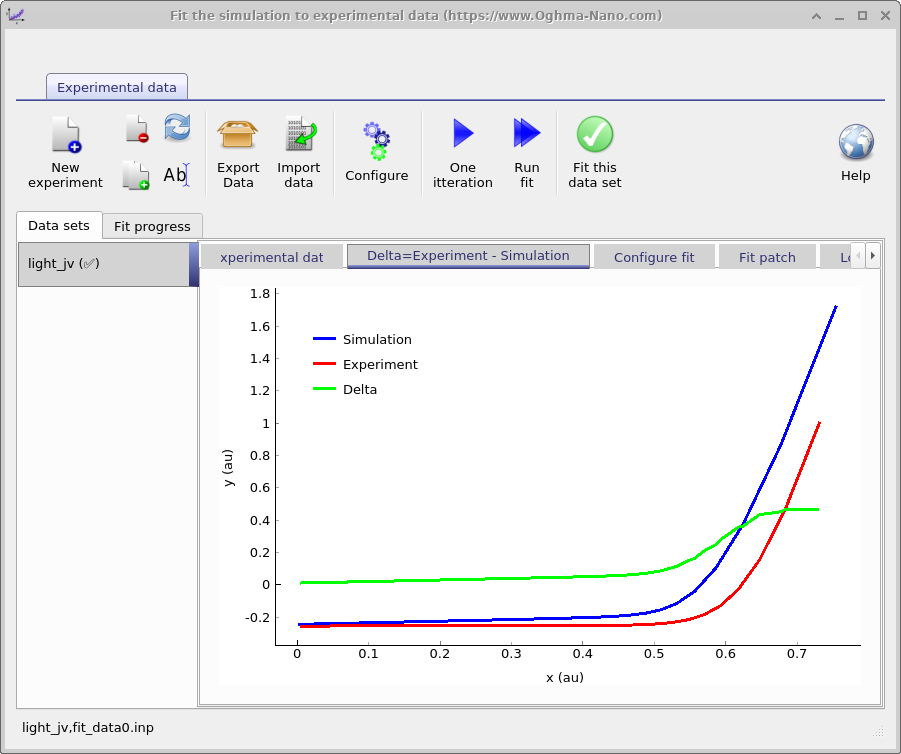
\includegraphics[width=0.45\textwidth]{./images/fit/fit_delta.png}
&
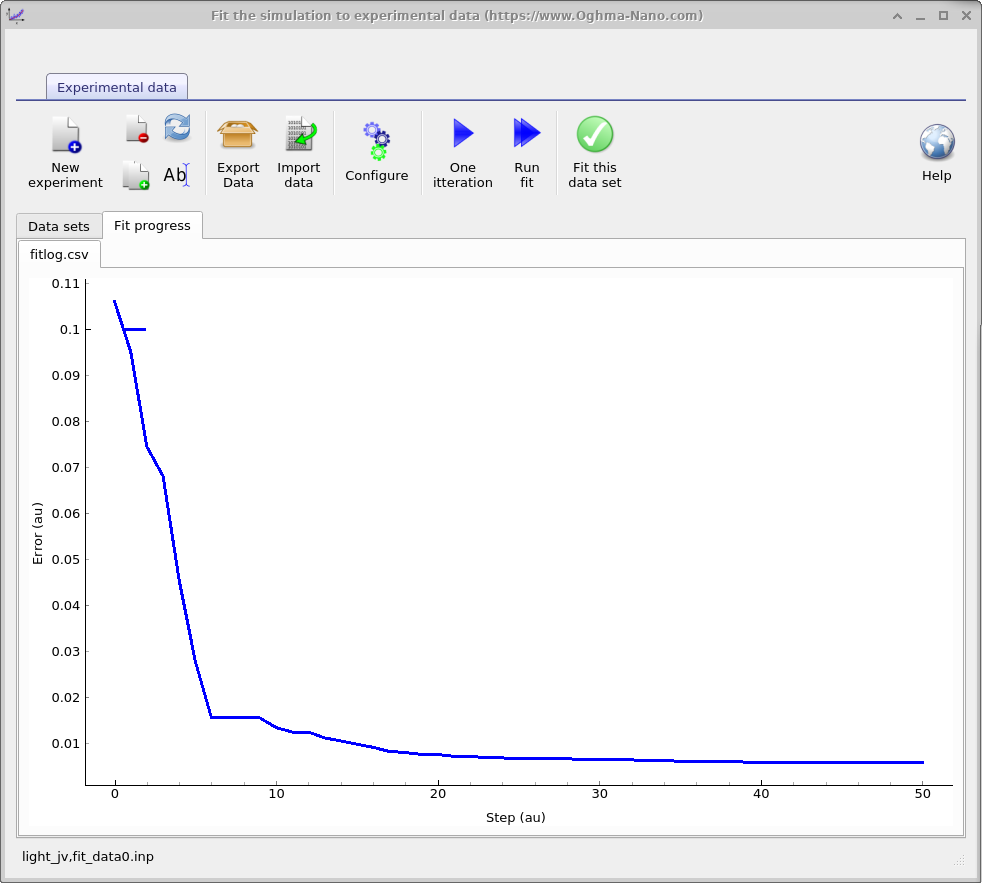
\includegraphics[width=0.45\textwidth]{./images/fit/fit_converge.png}
\\
\end{tabular}
\caption{a) The result of clicking the one fit button. b) The error function dropping during a simulation.}
\label{fig:fit_one_fit}
\end{figure}

\section{Setting the variables to fit}
In figure \ref{fig:fit_window_first_open}, there is a \emph{Configure} icon. If you click on this it will open the \emph{Fit variable window}.  This window is used to configure the fitting variables. The tab entitled \emph{Fit variables} defines the variables we will fit.  The more variables you fit at the same time the longer the fit will take. Try to minimize the number of variables you are fitting. A good tip is to start of fitting with symmetric parameters then only move to asymmetric parameters, once the fit becomes good. (see figure \ref{fig:fit_vars}).  You can see from Figure \ref{fig:fit_vars}, that there are 7 columns to the fit window, they have the following functions:

\begin{itemize}
  \item Enabled: This enables or disables the fitting of that variable.
  \item Variable: This describes the path of the variable to be fit in \emph{English}.
  \item Min: This is the minimum value the variable can take.
  \item Max: This is the maximum value the variable can take.
  \item Error function: If the variable strays out of the min-max range, this number will be added onto the total fitting error. This idea is this \emph{scares} the algorithm back into the allowed range.
  \item Log scale: This determines if the variable is fit on a log scale. For parameters which range over many orders of magnitude it is often useful to make sure the algorithm can explore the entire range.
  \item Variable (json): This is usually hidden, but represents the full path of the parameter to be fit in  \emph{json} format, it is this and not the \emph{English} path that is used by the back end. The \emph{English} path is generated for humans and can indeed not be correct as long as the json path is correct. 
\end{itemize}

\begin{figure}[H]
\centering
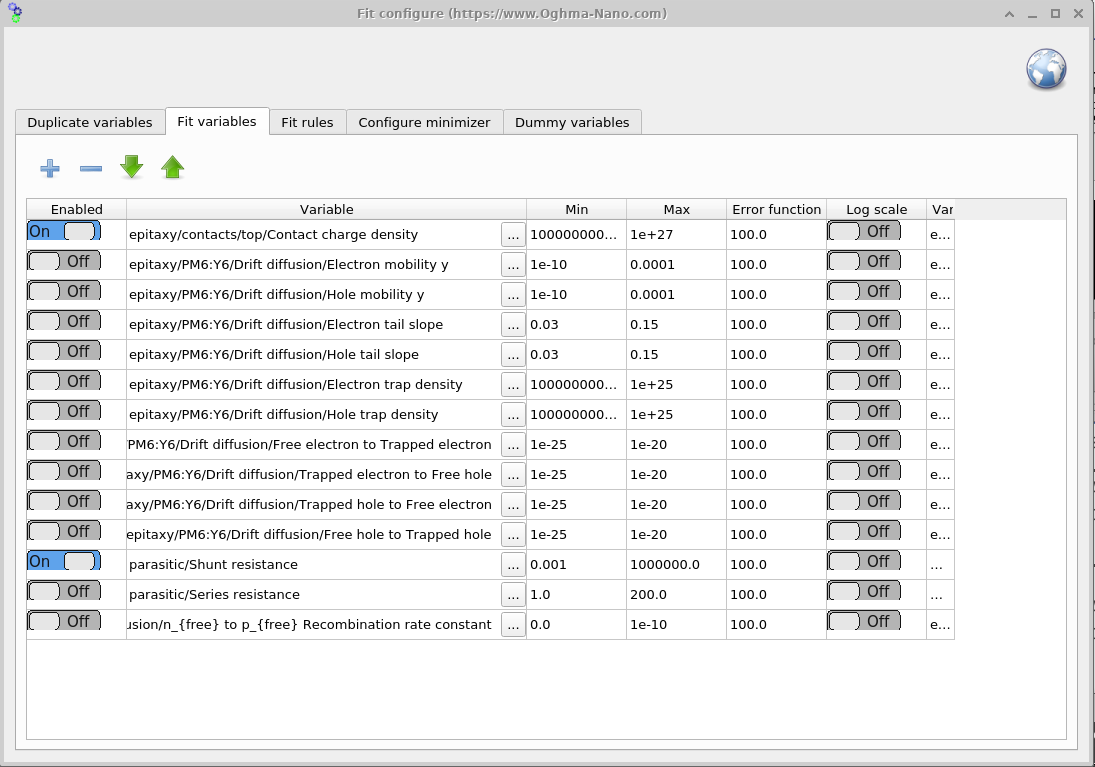
\includegraphics[width=0.7\textwidth]{./images/fit/fit_vars.png}
\caption{Defining the variables to fit and their ranges.}
\label{fig:fit_vars}
\end{figure}

\section{Duplicating variables}
The \emph{Fit Variable Window} includes a tab called \emph{Duplicate Variables}, which allows one parameter to be copied onto another. In this example, we assume the device is symmetric, meaning we only fit the electron parameter as a variable. However, we use the \emph{Duplicate Variables} tool to copy the newly fitted electron parameters onto the hole parameters. This approach enables us to vary electron mobility during the fitting process while ensuring that hole mobility maintains the same value at each step. (See Figure \ref{fig:fit_duplicate_vars}.)

If you examine the window closely, you will notice a column labeled "Function y=f(x)", where the default value is set to "x". This function defines how the source variable is transformed into the destination variable yy. For example, setting it to "2*x" would double the source variable each time it is copied. The available mathematical operations are detailed in Table \ref{sec:calculator}.

\begin{figure}[H]
\centering
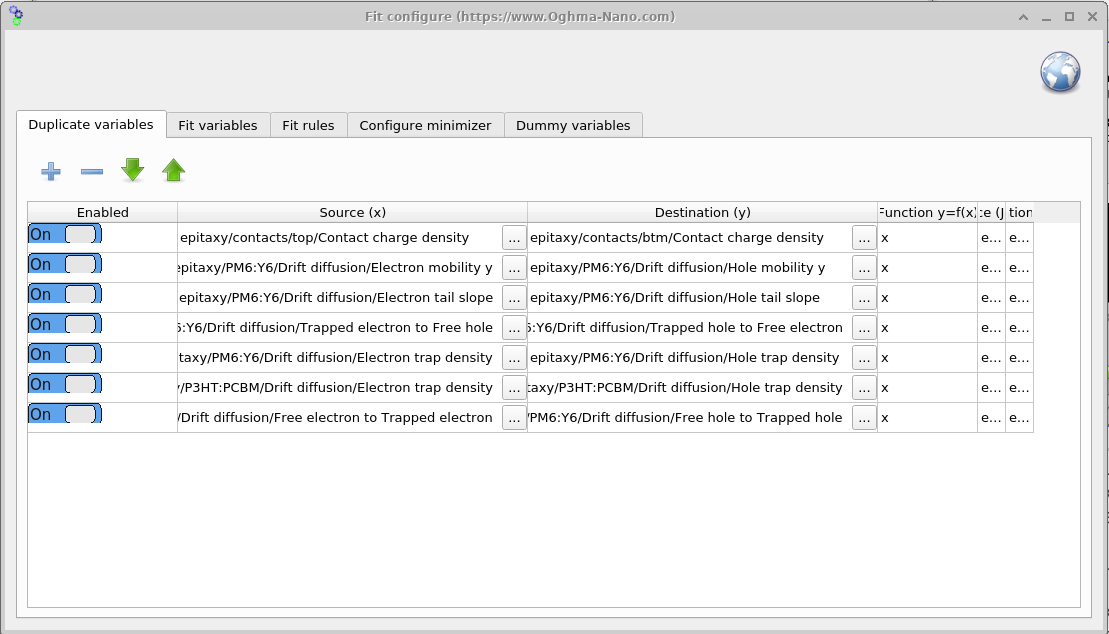
\includegraphics[width=0.7\textwidth]{./images/fit/fit_duplicate_vars.png}
\caption{Defining which variables are duplicated to other variables.}
\label{fig:fit_duplicate_vars}
\end{figure}


\section{Fit rules}
Also in the \emph{Fit variable window} is a tab called \emph{Fit rules}. This is used to enforce rules onto the fit, using mathematical expressions. For example one can force one parameter to always be bigger than another.

\section{Minimizer configuration}
Also in the \emph{Fit configure} window is a tab called \emph{Configure minimizer}. This configures the fitting algorithm that is used for the fit. Fitting algorithms are an entire research field in themselves. OghmaNano implements a few key algorithms to do the fitting. These are listed below. The algorithm used can be selected from the \emph{Fitting method} drop down box.
  
\begin{figure}[H]
\centering
\begin{tabular}{ c c }

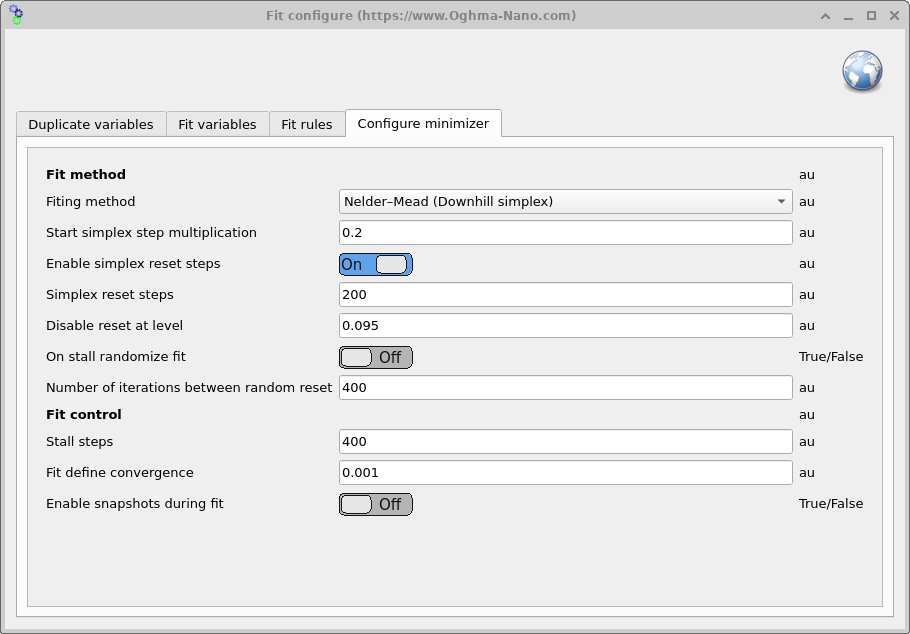
\includegraphics[width=0.45\textwidth]{./images/fit/configure_minimizer_simplex.png}
&
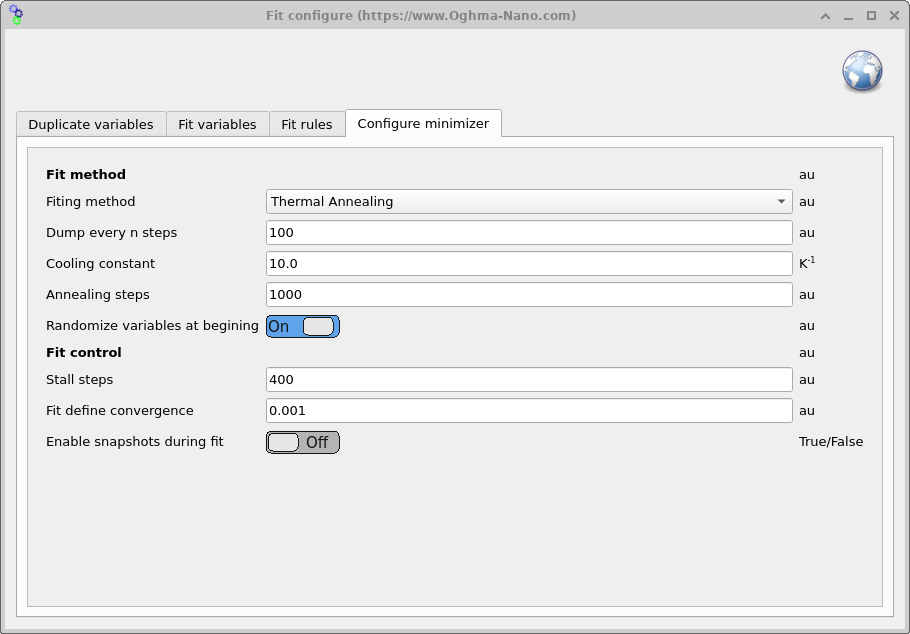
\includegraphics[width=0.45\textwidth]{./images/fit/configure_minimizer_thermal.png}
\\
\end{tabular}
\caption{a) Configuring the simplex downhill minimizer b) Configuring the thermal annealing minimizer.}
\label{fig:minimizer_config}
\end{figure}

There are in general two types of fitting algorithms. The first class of algorithms are gradient decent type, these attempt to effectively roll a ball down a hill to find the best fit. This class of algorithm can be divided into two sub types, ones which require the gradient to be calculated and those that do not. Calculating the gradient is computationally expensive and prone to errors with complex models. Therefore, generally more reliable fitting with methods that do not require the gradient to be explicitly calculate is usually more robust (in my exprience). The second class of algorithm are statistical methods, these methods have the advantage that the user does not only get a fit of the model to the data but a statistical distribution telling him/her how probable (and unique) the fit is. These methods therefore often require longer run times than down hill methods.

\begin{figure}[H]
\begin{tabular}{||c c c c c||} 
 \hline
 Method 				& Downhill	& Gradient &  Statistical & Comment\\ 
 \hline\hline
 Nelder-Mead			& x 		& 			&    & Robust, slow, reliable\\ 
 \hline
 Newton					& x 		&	x		&    & Fragile, sometimes fast\\
 \hline
 Thermal Annealing		&  			&			&  x & Surprisingly good\\
 \hline
 MCMC					&  			&			&  x & ?\\
 \hline
 HMC					&  			&			&  x & ?\\ [1ex] 
 \hline
\end{tabular}
\caption{Fitting methods implemented in OghamNano}
\label{tab:fitting_methods}
\end{figure}

\subsection{Nelder-Mead (Simplex Downhill)}
The simplex downhill algorithm is the most often used fitting method in OghmaNano, all papers published until 2024 used this method. More can be read about how the algroytham works here: \url{https://en.wikipedia.org/wiki/Nelder%E2%80%93Mead_method}. This minimizer has the following options: 

\begin{itemize}
  \item Stall steps: If fit error does not improve in this number of steps then the fit is considered stalled and therefore stopped.
  \item Disable reset at level: This will stop the fit restarting if fit error drops to below this level.
  \item Fit define convergence: This is the level of error at which the fit will stop.
  \item Start simplex step multiplication:  This defines the size of the first fitting step, a smaller value will mean the fitting algorithm will only change the initial numbers a bit, while a large number will change the initial numbers a lot. If you want your fit to explore the parameter space widely set this value to be greater than 1.0. If you want your fit to more or less stay around where your initial parameters are set this value to be less than 1.0.  A value of 2.0 is considered big, a value of 0.1 is considered small.
  \item Enable snapshots during fit: By default snapshots are turned off during fitting as they produce a lot of disk access to allow them the be dumped to disk set this on.
  \item Simplex reset steps: This sets after how many steps the simplex algorithm is reset. Resetting the algorithm can push the answer away from the solution, but it can also pop the solver out of a valley if it has become trapped and allow better convergence.
\end{itemize}

The advantage of this method is that it effectively looks for an answer by rolling a ball down hill. It also does not need to take gradients of the problem, which can be beneficial in complex problem spaces.

\subsection{Newton}
Newton's method is included for completeness. In my experience it is quite unstable when used with fitting. This is a gradient method, thus requires derivatives to be calculated. This can make the fitting process unstable, but the advantage is that it can be faster than Nelder-Mead in some circumstances for some classes of problem.

\subsection{Thermal Annealing}
This is a classical thermal annealing algorithm. The algorithm will only explore the parameter space defined by the allowed limits of the fit variables, thus to use this efficiently it is key to set these limits correctly. I have found this method to be surprisingly good and often faster than Nelder-Mead, however the final results are often not as polished as those for Nelder-Mead.

\begin{itemize}
  \item Dump every n steps: Writes the output to disk every n steps
  \item Cooling constant: Defines how quickly the problem cools, the cooling takes the form of $e^{-k(T_{start}-T_{stop})}$, where $T_{start}$ is 300K and $T_{stop}$ is 0K.
  \item Annealing steps: Defines the number of steps taken to get from $T_{start}$ to $T_{stop}$. 
\end{itemize}

\subsection{Markov chain Monte Carlo (MCMC)}
This method is under development.

\subsection{Hamiltonian Monte Carlo (HMC)}
This method is under development.

\subsection{No-U-Turn Sampler (NUTS)}
This method is under development.



\section{How the fitting process works}
When you click the "Run fit" button, OghmaNano makes a new directory inside the simulation directory called "sim" this is the directory in which the fitting process takes place. Inside this directory OghmaNano will make one new directory for each data set you are trying to fit, it will populate each directory with the sim.json (and sim.oghma) files from your main simulation directory.  At this point the sim.json files in all the directories are identical.  Then using the contents of the fit "fit patch" (see figure \ref{fig:fit_patch}) the content of each sim.json file will be updated, this process is called patching the simulation files.  This process enables you to adjust parameters in each simulation directory to match the data set you are trying to fit. For example you might want one data set to have optical/light/Psun set 1.0 and another to be set to 0.0 to enable fitting of a 1 sun JV curve and a dark JV curve. After patching each directory, the fitting process then commences. During this process fitting variables in the sim.json files in the "sim" directory are updated.  During the fit the algorithm will often produce fits which are worse than the current best effort, and only sometimes produce fits which are better than the current best effort. Only when a better fit is obtained will the sim.json file be updated in the main simulation directory and the curves in the GUI also updated.

\begin{figure}[H]
\centering
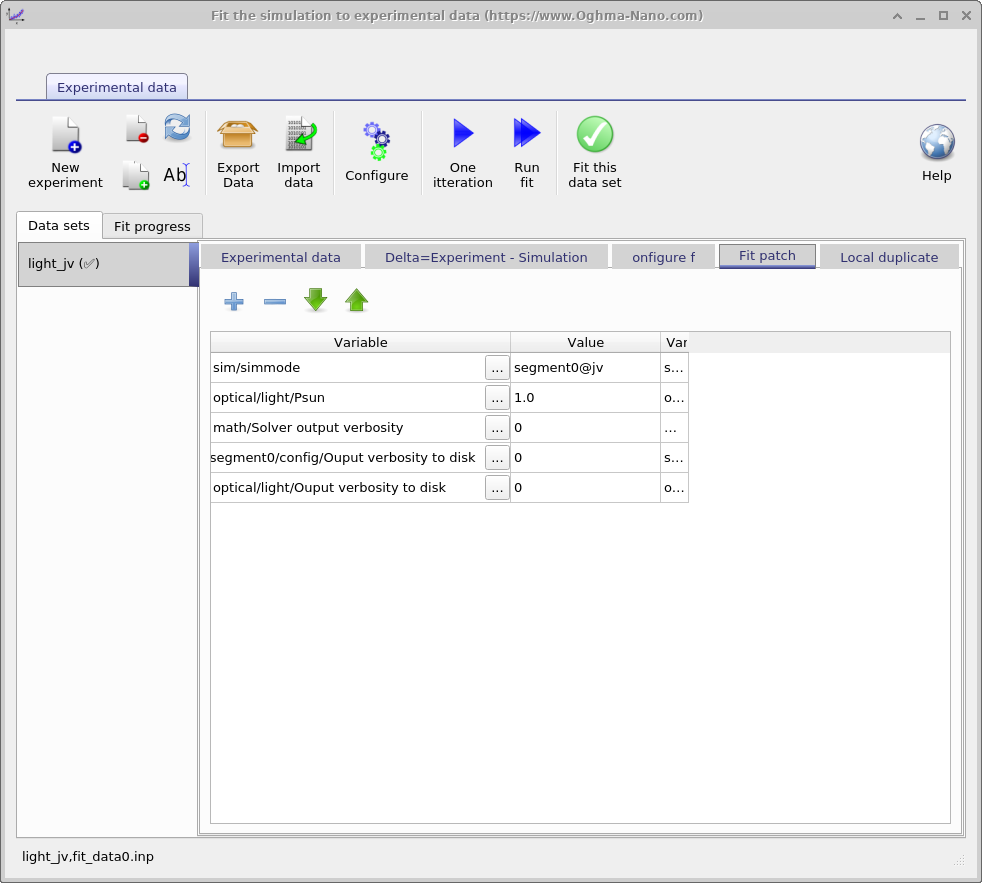
\includegraphics[width=\textwidth]{./images/fit/fit_patch.png}
\caption{The fit patch applied to each data set.}
\label{fig:fit_patch}
\end{figure}


\section{Fitting without the GUI}
The GUI is a very easy and efficient way to setup a fit. However, it takes considerable CPU time to update the user interface as the fit runs and this therefore slows the fitting process. Therefore if you are doing lots of fitting or fitting difficult problems, fitting without the GUI can be faster.  This section covers how to fit from the Windows command line:

\begin{enumerate}
  \item First set up your simulation you want to fit in the usual way using the GUI. Run a single iteration of the fit to make sure it looks right.  Then close the GUI.
  \item Next we need to tell Windows where it can find OghmaNano, usually it has been installed in C:\textbackslash Program files x86 \textbackslash OghmaNano . If you open this directory you will see lots of files.  But the two key ones are \emph{oghma.exe} and \emph{oghma\_core.exe}. The file \emph{oghma.exe} is the GUI, \emph{oghma\_core.exe} is the core solver, these are completely independent programs.  The core solver can be run without the GUI.  To tell windows where these files are we need to add C:\textbackslash Program files x86 \textbackslash OghmaNano to the windows path. This can be done by following these \url{https://docs.microsoft.com/en-us/previous-versions/office/developer/sharepoint-2010/ee537574(v=office.14)} instructions.  These instructions are for a modern version of Windows, but on your system things may be in slightly different places. On most versions of windows the process is more or less the same, if you get stuck google "adding a path to window".

  \item Click on the start menu and type "cmd" and enter to bring up a Windows terminal.  Type:
\begin{listing}[H]
\begin{minted}[frame=single,
               framesep=3mm,
               linenos=false,
               xleftmargin=21pt,
               tabsize=4]{bash}
oghma_core.exe --help
\end{minted}
\end{listing}
Note it is a double dash before help not a single dash.

This should bring up some help for OghmaNano.  If it does them we have successfully told windows where \emph{oghma\_core.exe} lives. If you get an error, try step 2 again (and/or restart your computer).
  \item Now that windows knows where \emph{oghma\_core.exe} lives, we can navigate to our simulation directory.  Use \emph{cd} to navigate to the directory where your simulation you want to fit is saved.
  \item First run the command \emph{oghma\_core.exe} to see if your simulation runs OK. If it does not then recheck your simulation file.
  \item Now run a single fit by typing:

\begin{listing}[H]
\begin{minted}[frame=single,
               framesep=3mm,
               linenos=false,
               xleftmargin=21pt,
               tabsize=4]{bash}
oghma_core.exe --1fit
\end{minted}
\end{listing}

Inspect the results in the "sim" directory, use your favourite plotting program to compare the results to the experimental data. Note the experimental data is stored in \emph{fit\_data(0-1).inp}.

  \item If everything went well with the above step, you can run a real fit by typing:
\begin{listing}[H]
\begin{minted}[frame=single,
               framesep=3mm,
               linenos=false,
               xleftmargin=21pt,
               tabsize=4]{bash}
oghma_core.exe --fit
\end{minted}
\end{listing}
Again those are double dashes before the fit command. Ctrl+C will terminate the fit. You can check the progress of convergence by plotting \emph{fitlog.csv}.

\end{enumerate}





